\documentclass[oneside]{abntex2}
\usepackage[utf8]{inputenc}
\usepackage{courier}
\usepackage{graphicx}
\usepackage{amsmath}
\usepackage{amssymb}
\usepackage{subcaption}

\title{Relatório do Segundo Trabalho de Algoritmos Numéricos}
\author{Gabriel Pietroluongo Nascimento}
\date{2019}
\local{Universidade Federal do Espírito Santo}

\begin{document}
%\maketitle
\imprimircapa
\tableofcontents
\chapter{Introdução}
\section{Objetivo} \label{sec_obj}
Este trabalho tem como objetivo a solução da equação de Poisson pelo método das diferenças finitas centrais, com o sistema resultante sendo resolvido pelo método SOR. Com isso, é possível testar o sistema resultante com uma solução conhecida ou propor uma modelagem aproximada de um problema com comportamento conhecido sem solução exata conhecida. Para isso, foi proposta uma especificação técnica para a implementação de um sistema que resolva problemas que possam ser modelados dessa forma, dado um conjunto de dados em forma de uma função aproximante e um determinado número de casos de contorno, aproximando o resultado gerado do resultado real. 

\section{Método de Poisson} \label{sec_method}
Para a aplicação do método de Poisson, é considerado um domínio $\Omega = [a, b]\times[c, d]$, com fronteira descrita por $\partial{\Omega}$ de forma que

\begin{equation}
\label{poissond}
    f(x, y) = - \left(\frac{\partial^2{V}}{\partial{x^2}} + \frac{\partial^2{V}}{\partial{y^2}}\right)
\end{equation}

\begin{equation}
\label{poissonbd}
    g(x, y) = V
\end{equation}

Com isso, temos que a equação \ref{poissond} é a definição para $x, y$ dentro do domínio $\Omega$ do sistema e a equação \ref{poissonbd} é a definição para $x, y$ na fronteira do domínio. Além disso, $f(x,y)$ e $g(x,y)$ são funções conhecidas. O objetivo do método é determinar uma função $V(x,y)$ no interior do domínio $\Omega$, utilizando subdivisões do domínio em células retangulares pelo método das diferenças finitas. Após essa segmentação o resultado será um sistema linear, que será resolvido neste projeto por meio do método SOR.

A discretização da equação de Poisson por diferenças finitas centrais pode ser escrita em termos de constantes $a, b, c, d, e$ de forma que a expressão no ponto $(i,j)$, ou seja, sendo $f$ o vetor de solução do sistema, $f_{ij}$, seja:
\begin{equation}
    f_{ij} = aV_{(i+1), j} + bV_{(i-1), j} + cV_{i, (j+1)} + dV_{i, (j-1)} + eV_{ij}
\end{equation}
onde as constantes $a, b, c, d, e$ são dadas por

\begin{equation}
\label{eqConstAB}
    a = b = \frac{-1}{h_x^2}
\end{equation}
\begin{equation}
\label{eqConstCD}
    c = d = \frac{-1}{h_y^2}
\end{equation}
\begin{equation}
\label{eqConstE}
    e = 2 \cdot \left(\frac{1}{h_x^2} + \frac{1}{h_y^2}\right)
\end{equation}

Com o cálculo dessas constantes e uma matriz $f$ que consiste no cálculo de $f(x, y) $ para todo $x, y$ no domínio de análise, é possível calcular pelo método SOR uma matriz-solução V, de $i = n_x \cdot n_y$ elementos, no qual cada elemento $V_i$ é dado pela equação

\begin{equation}
\label{eqSORMain}
    V_i = \frac{\omega}{e} \cdot (f_i - dV_{i-n_x} - bV_{i-1} - aV_{i+1} - cV_{i+n_x}) + (1-\omega)V_i
\end{equation}

Com isso, é possível iterar nos termos do vetor $V$ e aproximar os valores do valor exato da função real. Por fim, é necessário considerar casos de contorno, caso existam, nas iterações do SOR. 
\chapter{Desenvolvimento do projeto}

\section{Implementação do Projeto} \label{sec_impl}
Para o desenvolvimento do projeto, a linguagem escolhida foi C++, por conta da robustez no processamento e das características de orientação a objetos que possibilitam uma generalização das aplicações do sistema, não limitando ele a apenas os problemas apresentados na especificação. 

\subsection{Implementação do algoritmo}
Conforme descrito na seção anterior, o algoritmo de Poisson foi implementado para solucionar o sistema proposto. Para isso, seguindo a especificação do trabalho, primeiramente foram definidos $h_x$ e $h_y$ para analisar os resultados em diferentes malhas. Assim, o algoritmo foi testado com $h_x = h_y = 0.5, 0.25, 0.125$, e os resultados obtidos comparados. Com esses valores, é possível definir a quantidade de subintervalos $n_x$ e $n_y$ seguindo as seguintes equações:
\begin{equation}
    n_x = 1 + \frac{(b-a)}{h_x}    
\end{equation}
e
\begin{equation}
    n_y = 1 + \frac{(d-c)}{h_y}
\end{equation}
com $a, b, c, d$ sendo os limites do domínio tal que $\Omega = [a, b] \times [c, d] $. Após a definição desses valores, foi definido um $\omega$ seguindo a equação 

\begin{equation}
\label{eqOmega}
    \omega = \frac{8-\sqrt{64-16t^2}}{t^2}
\end{equation}
onde
\begin{equation}
\label{eqOmegaT}
    t = \cos{\left(\frac{\pi}{n_x}\right)} + \cos{\left(\frac{\pi}{n_y}\right)}
\end{equation}
conforme proposto no material de apoio. Com isso, temos o domínio discretizado na forma $\Omega = \{(x, y) | a<x<b, c<y<d\}$.

Com esses valores, é possível calcular os valores das constantes $a, b, c, d, e$ por meio das equações \ref{eqConstAB}, \ref{eqConstCD} e \ref{eqConstE}. Seguindo o modelo proposto, também foi preenchida a matriz $f$ com os valores de $f(x,y)$, conforme descrito na seção \ref{sec_method}. Nessa etapa, também são aplicadas as condições de contorno da função descritiva no vetor $f$, antes da aplicação do método SOR. Caso tenha sido providenciada uma função de validação (solução exata), esse ponto do código seria o ideal para o preenchimento da matriz de soluções exatas, chamada daqui para a frente de \textit{matriz ground-truth} e representada por $q$. Com todos esses elementos preparados, é possível aplicar a solução via SOR seguindo a equação \ref{eqSORMain} até um máximo de iterações predefinido, completando o algoritmo e produzindo o resultado aproximado da função original. Posteriormente, é possível comparar o erro do método utilizando a equação sugerida pela especificação do projeto, 

\begin{equation}
\label{eqError}
    \epsilon = max|q_i - v_i|, 0<v<(n_x \cdot n_y) - 1
\end{equation}

Analisando o erro, é possível definir a qualidade da aproximação do sistema, dependendo de quanta precisão é necessária pelo sistema.

\subsection{Escrita inicial do algoritmo} \label{subsec_alg_init}
Para o desenvolvimento projeto, inicialmente foi implementado um algoritmo "cru" em C++, seguindo o processo descrito na seção \ref{sec_impl}. De posse desse algoritmo inicial, foi possível testar a implementação e obter um resultado de acordo com o esperado pela especificação do projeto (erro menor que $10^{-6}$). Além disso, foram testados vários valores de iterações e de passos, a fim de verificar se a solução seria aplicável em mais de um caso e garantir que não haviam \textit{bugs} no projeto. Uma mudança em relação ao material de apoio foi que os "casos de contorno" do método SOR não foram calculados seguindo a especificação, mas sim analisando quais seriam os problemas enfrentados a cada iteração\footnote{Isso é necessário pois o algoritmo apresentado originalmente considera que apenas multiplicar o resultado por 0 já seria o suficiente para evitar problemas de \textit{overflow} / \textit{underflow}. Contudo, como em C++ o acesso a memória em regiões impróprias não tem comportamento definido, é mais prudente analisar cada caso separadamente e evitar problemas de manipulação de memória indevida}. Com isso, a cada iteração do SOR, o cálculo dos termos utilizando a equação \ref{eqSORMain} é considerada separadamente, e cada um dos termos que poderia ter problemas de memória é analisado individualmente. Considerando que o algoritmo inicial foi uma versão mais direta, o conteúdo dele é praticamente uma aplicação direta do algoritmo mencionado anteriormente, com a exceção mencionada acima, e com o uso de variáveis globais e outros artefatos da linguagem que facilitam a prototipagem de ideias mas em longo prazo atrapalham o desenvolvimento. Assim, esse código de qualidade menor foi analisado, otimizado e reescrito para a aplicação final no projeto.

\subsection{Implementação da classe}
De posse do algoritmo já escrito na linguagem-alvo, o código teria que ser reescrito para melhorar sua legibilidade e expansibilidade (já que deve ser utilizado para resolver mais de um único problema). Com isso, primeiramente todos os valores que antes eram \textit{"hardcoded"} em seu interior foram substituídos por variáveis apropriadas. Os métodos foram analisados e uma classe em C++, \textit{poissonSOR} foi criada para resolver os problemas modelados da forma proposta. Com isso, é possível apenas passando parâmetros e reimplementando pequenos pedaços de código (casos de contorno) utilizar a implementação base para qualquer problema do tipo sugerido. De fato, todos os problemas do projeto tiveram sua solução decorrente da aplicação direta da classe escrita. Isso viabiliza um fluxo de trabalho mais elegante, à medida que uma análise de um fenômeno diferente modelado seguindo a equação de Poisson pode ser implementado rapidamente utilizando o código mais complexo, já escrito, como base. As minúcias dos métodos e atributos da classe implementada estão descritos em profundidade na seção \ref{sec_doc}.

\subsection{Geração de saídas}
O código em C++ faz o processamento e salva o resultado em arquivos no formato \textit{.txt} na pasta do programa. Com esses dados já processados, um \textit{script} em \textit{Python} foi desenvolvido para a geração dos dados de saída apresentados no capítulo \ref{sec_conc}, utilizando algumas bibliotecas próprias da linguagem, como \textit{matplotlib} e \textit{numpy}. Assim, dado um conjunto de dados de determinado problema e as informações sobre esse conjunto, ou seja: se $f_{[i\times j]}$ é o conjunto, dados todos os elementos $f_{ij}$ e $i, j$, é possível gerar o mapa de potenciais (\textit{heatmap}) bidimensional e tridimensional e de linhas equipotenciais do conjunto de dados.

\section{Dificuldades encontradas}
As principais dificuldades encontradas no projeto foram determinar a abordagem adequada e como organizar os códigos escritos em termos de paradigmas de programação, ou seja, se seriam utilizadas classes puras de C++ ou apenas \textit{structs} simples de C, ou até mesmo apenas uma única função que resolveria um sistema nesse formato. Com isso, para possibilitar a entrega do trabalho no prazo especificado, uma abordagem \textit{top-down} foi adotada, isto é, ao invés de focar na base do código, o foco foi alterado para obter um resultado por meio do algoritmo "cru" desenvolvido, conforme descrito anteriormente. Isso viabilizou um desenvolvimento mais rápido por não ser necessário implementar políticas de acesso (como membros privados/públicos) inicialmente, apenas na etapa de "tradução" do código original para o paradigma orientado a objetos. Considerando isso tudo, a escolha por classes no paradigma orientado a objetos foi feita pela necessidade de analisar mais de um problema do mesmo tipo, conforme descrito na especificação, e pela praticidade de reutilização de código decorrente desse paradigma. Com isso, é possível utilizar de forma eficiente todos os scripts escritos, mesclando a parte estática de cada problema individual (como domínio e função aproximante) com o componente comum (método SOR e cálculos de erros, por exemplo). Dessa forma, mesmo que fosse necessário resolver mais um problema diferente, com um domínio diferente e com uma função e casos de contornos diferentes, seria possível implementar apenas uma "expansão" ao código já existente e obter um resultado.

Outra dificuldade foi a implementação dos casos de contorno no algoritmo SOR, o que tomou grande parte do tempo de desenvolvimento. Com a abordagem tomada, isso não deve ser mais um problema futuro, considerando que a classe implementada deixa bem claro ao cliente como implementar os casos de contorno de forma eficaz. Os casos de borda do algoritmo SOR também tomaram grande parte do tempo de desenvolvimento do projeto, tendo em vista a dificuldade para analisar resultados que são decorrentes de \textit{lixo} na memória do computador, conforme descrito na seção \ref{subsec_alg_init}.

\chapter{Conclusão} \label{sec_conc}
\section{Resultados}
Primeiramente, é necessário definir um número máximo de iterações realizadas. Para isso, foi realizado um estudo do erro em função da quantidade de iterações realizadas. O erro $V_p$ é dado pela equação \eqref{eqError}, e se refere ao resultado dos potenciais. O erro do campo elétrico é calculado de forma similar. Para cada teste, os valores de passo foram definidos como $h_x = h_y = p$, que será a nomenclatura utilizada na seção de conclusão do projeto. Com isso, as informações sobre o estudo feito estão dispostas abaixo:

\begin{table}[h]
    \centering
    \begin{tabular}{c|c|c}
    Número de iterações &Erro $V_p$ &Erro Campo Elétrico  \\
    \hline
    1 & 12.538790426611 & 2.907351752175 \\
    10 & 0.191925842523 & 0.077129816371 \\
    20 & 0.006512396150 & 0.004120976576 \\
    30 & 0.000286799515 & 0.000160785244 \\
    40 & 0.000001920159 & 0.000000852291 \\
    50 & 0.000000014172 & 0.000000006622 \\
    60 & 0.000000000092 & 0.000000000064 \\
    70 & 0.000000000003 & 0.000000000001 \\
    80 & 0.000000000000 & 0.000000000000 \\
    90 & 0.000000000000 & 0.000000000000 \\
    100 & 0.000000000000 & 0.000000000000 \\
    \end{tabular}
    \caption{Análise da validação com $p = 0.5$ e 12 casas decimais de precisão}
    \label{tab:iter_p05}
\end{table}


\begin{table}[h]
    \centering
    \begin{tabular}{c|c|c}
    Número de iterações &Erro $V_p$ &Erro Campo Elétrico  \\
    \hline
    1 & 14.167268340547 & 1.738923212435 \\
    15 & 0.460664261978 & 0.104090120849 \\
    30 & 0.029494914215 & 0.006383550807 \\
    45 & 0.002814599292 & 0.000791168413 \\
    60 & 0.000243688702 & 0.000048514634 \\
    75 & 0.000008360406 & 0.000001642513 \\
    90 & 0.000000049337 & 0.000000010677 \\
    105 & 0.000000001328 & 0.000000000288 \\
    120 & 0.000000000080 & 0.000000000015 \\
    135 & 0.000000000003 & 0.000000000001 \\
    150 & 0.000000000000 & 0.000000000000 \\
    \end{tabular}
    \caption{Análise da validação com $p = 0.25$ e 12 casas decimais de precisão}
    \label{tab:iter_p025}
\end{table}

\begin{table}[h]
    \centering
    \begin{tabular}{c|c|c}
    Número de iterações &Erro $V_p$ &Erro Campo Elétrico  \\
    \hline
    1 & 14.921764813058 & 0.928441841153 \\
    30 & 0.504155358122 & 0.059665023973 \\
    60 & 0.028215890019 & 0.002967654161 \\
    90 & 0.003017518043 & 0.000355706314 \\
    120 & 0.000220905358 & 0.000018882376 \\
    150 & 0.000006437956 & 0.000000483484 \\
    180 & 0.000000035639 & 0.000000003380 \\
    210 & 0.000000001213 & 0.000000000083 \\
    240 & 0.000000000052 & 0.000000000003 \\
    270 & 0.000000000001 & 0.000000000000 \\
    300 & 0.000000000000 & 0.000000000000 \\
    \end{tabular}
    \caption{Análise da validação com $p = 0.125$ e 12 casas decimais de precisão}
    \label{tab:iter_p0125}
\end{table}

\newpage

Analisando as tabelas apresentadas, é possível perceber que a partir de 300 iterações, o erro cometido é mínimo, mesmo com uma malha de alta resolução, com $p=0.125$. Portanto, os próximos resultados apresentados foram gerados utilizando esse número de iterações.

Para gerar os resultados demonstrados abaixo, todos os casos de teste foram rodados com o número máximo de iterações definido em 70, conforme exposto acima. Nessas condições, os seguintes resultados foram obtidos:

\begin{figure}[h]
  \begin{subfigure}[b]{0.5\textwidth}
    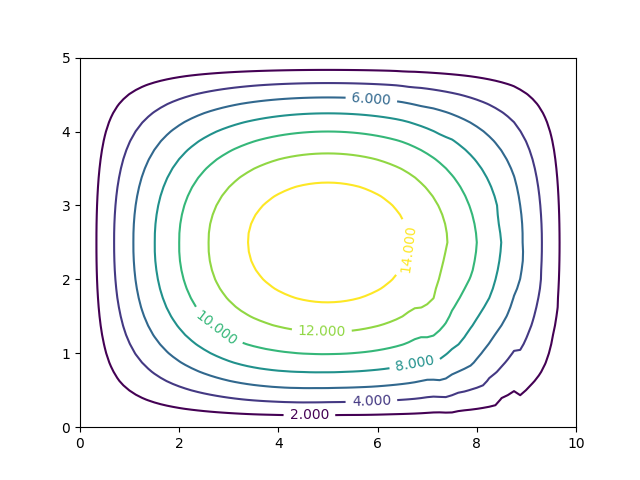
\includegraphics[width=\textwidth]{imgs/cont_aprox_val_1250.png}
    \caption{Aproximação do sistema com passo $p = 0.125$}
    \label{cont_aprox_val_1250}
  \end{subfigure}
  %
  \begin{subfigure}[b]{0.5\textwidth}
    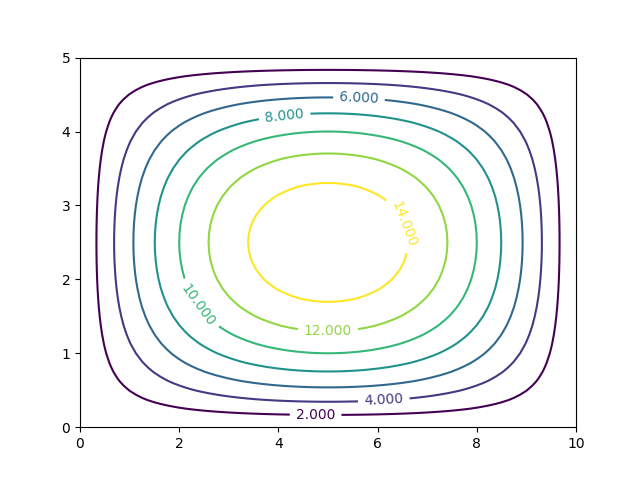
\includegraphics[width=\textwidth]{imgs/cont_grnd_val_1250.png}
    \caption{Resultado exato com passo $p = 0.125$}
    \label{cont_exat_val_1250}
  \end{subfigure}
  \caption{Mapa de linhas equipotenciais do sistema de validação}
\end{figure}

\begin{figure}[h]
  \begin{subfigure}[b]{0.5\textwidth}
    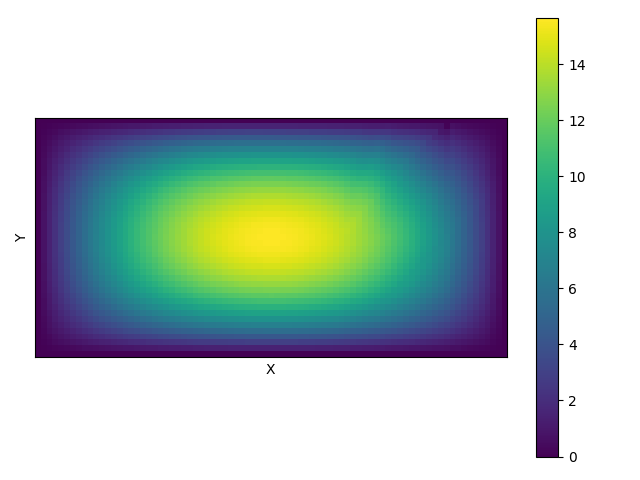
\includegraphics[width=\textwidth]{imgs/hmap_aprox_val_1250.png}
    \caption{Aproximação do sistema com passo $p = 0.125$}
    \label{hmap_aprox_val_1250}
  \end{subfigure}
  %
  \begin{subfigure}[b]{0.5\textwidth}
    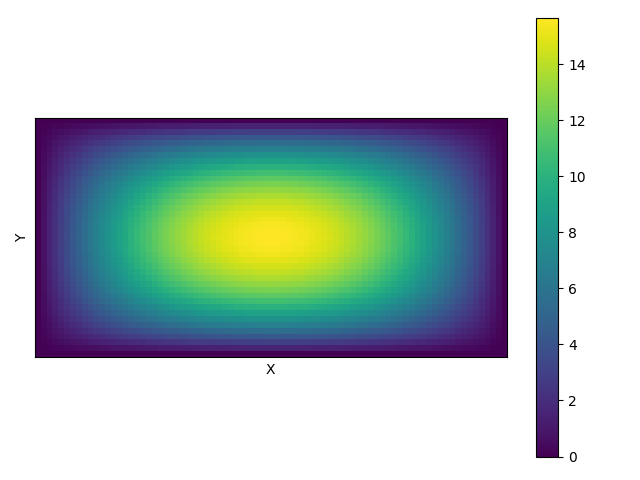
\includegraphics[width=\textwidth]{imgs/hmap_grnd_val_1250.png}
    \caption{Resultado exato com passo $p = 0.125$}
    \label{hmap_exat_val_1250}
  \end{subfigure}
  \caption{Mapa bidimensional dos potenciais do sistema de validação}
\end{figure}

\begin{figure}[h]
  \begin{subfigure}[b]{0.5\textwidth}
    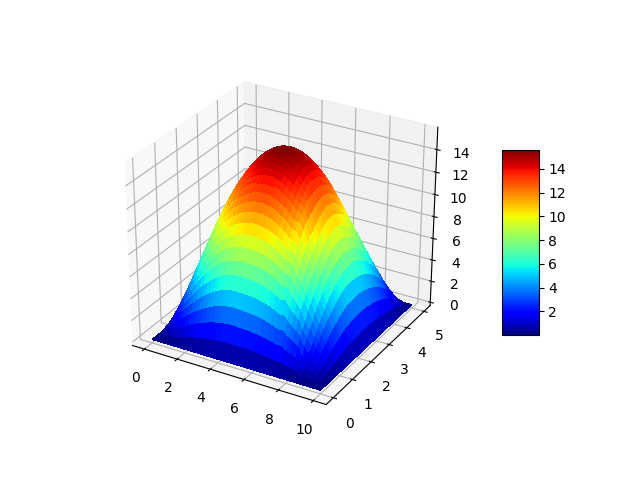
\includegraphics[width=\textwidth]{imgs/3d_aprox_val_1250.png}
    \caption{Aproximação do sistema com passo $p = 0.125$}
    \label{3d_aprox_val_1250}
  \end{subfigure}
  %
  \begin{subfigure}[b]{0.5\textwidth}
    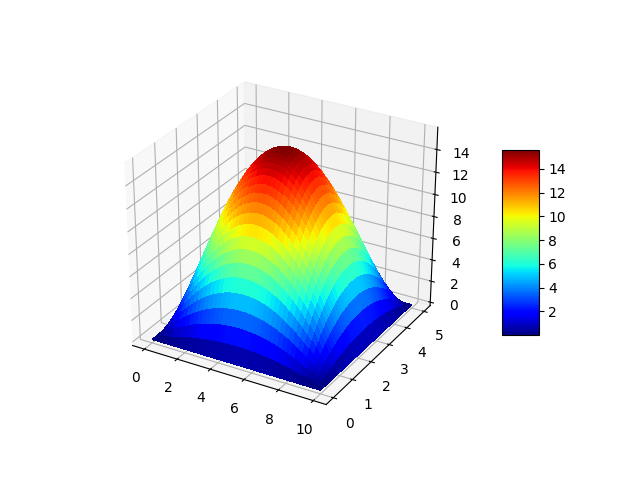
\includegraphics[width=\textwidth]{imgs/3d_grnd_val_1250.png}
    \caption{Potenciais exatos com passo $p = 0.125$}
    \label{3d_exat_val_1250}
  \end{subfigure}
  \caption{Modelo 3D dos potenciais do sistema de validação}
\end{figure}

\newpage

Além da análise dos potenciais do sistema, também foi analisado o campo elétrico:

\begin{figure}[h]
  \begin{subfigure}[b]{0.5\textwidth}
    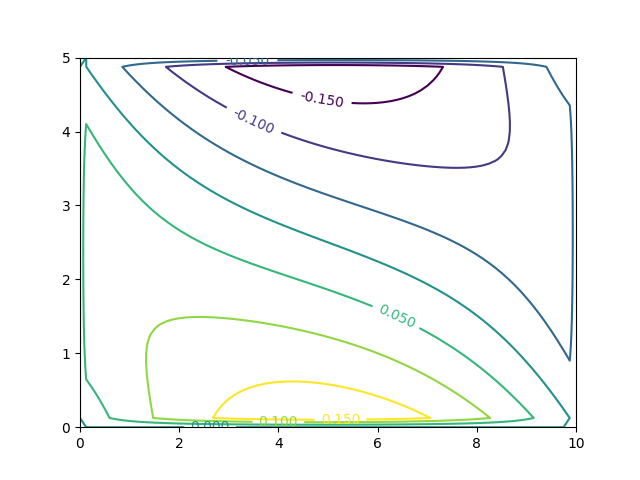
\includegraphics[width=\textwidth]{imgs/cont_aprox_val_elet_1250.png}
    \caption{Aproximação do sistema com passo $p = 0.125$}
    \label{3d_aprox_val_1250}
  \end{subfigure}
  %
  \begin{subfigure}[b]{0.5\textwidth}
    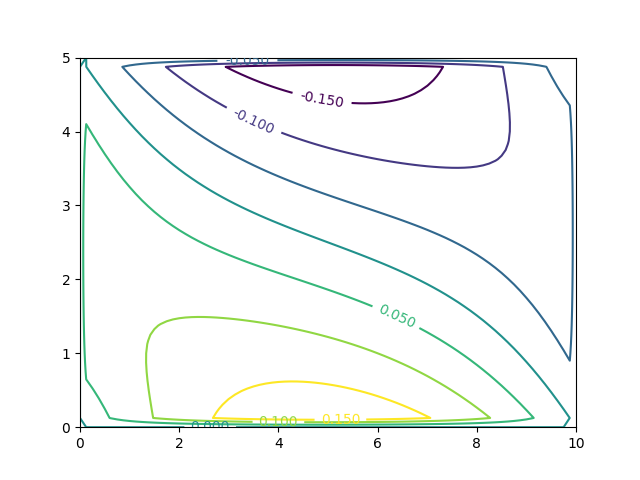
\includegraphics[width=\textwidth]{imgs/cont_grnd_val_elet_1250.png}
    \caption{Campo elétrico exato com passo $p = 0.125$}
    \label{3d_exat_val_1250}
  \end{subfigure}
  \caption{Modelo 3D dos campos elétrico do sistema de validação}
\end{figure}

\begin{figure}[h]
  \begin{subfigure}[b]{0.5\textwidth}
    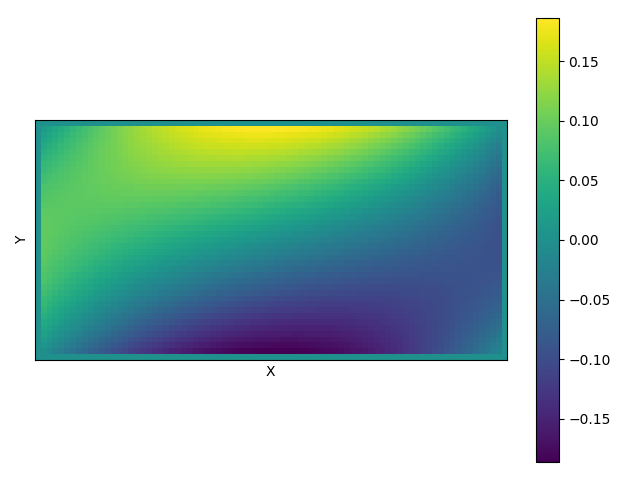
\includegraphics[width=\textwidth]{imgs/hmap_aprox_val_elet_1250.png}
    \caption{Aproximação do sistema com passo $p = 0.125$}
    \label{3d_aprox_val_1250}
  \end{subfigure}
  %
  \begin{subfigure}[b]{0.5\textwidth}
    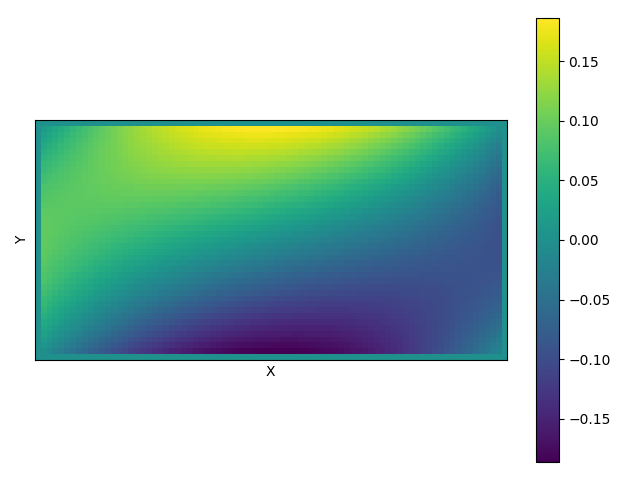
\includegraphics[width=\textwidth]{imgs/hmap_grnd_val_elet_1250.png}
    \caption{Campo elétrico exato com passo $p = 0.125$}
    \label{3d_exat_val_1250}
  \end{subfigure}
  \caption{Modelo 3D dos campos elétrico do sistema de validação}
\end{figure}


\begin{figure}[h]
  \begin{subfigure}[b]{0.5\textwidth}
    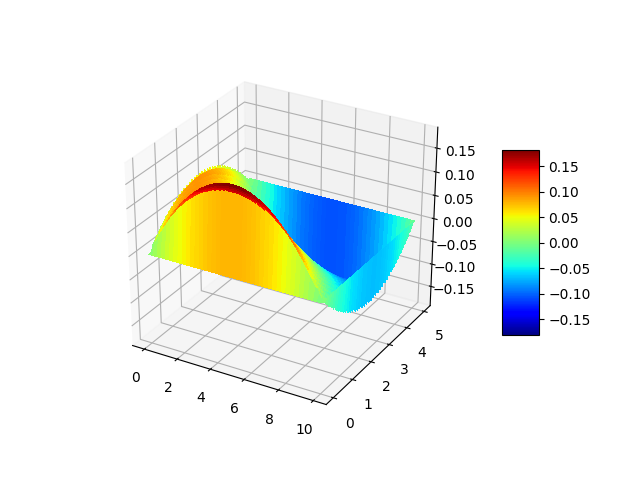
\includegraphics[width=\textwidth]{imgs/3d_aprox_val_elet_1250.png}
    \caption{Aproximação do sistema com passo $p = 0.125$}
    \label{3d_aprox_val_1250}
  \end{subfigure}
  %
  \begin{subfigure}[b]{0.5\textwidth}
    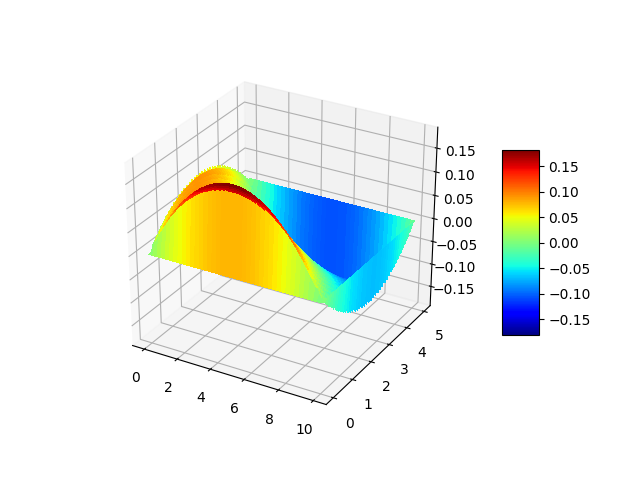
\includegraphics[width=\textwidth]{imgs/3d_grnd_val_elet_1250.png}
    \caption{Campo elétrico exato com passo $p = 0.125$}
    \label{3d_exat_val_1250}
  \end{subfigure}
  \caption{Modelo 3D do campo elétrico do sistema de validação}
\end{figure}

\newpage
Além dos casos de validação expostos acima, também foi analisado o sistema de capacitores:

\begin{figure}[h!]
    \centering
    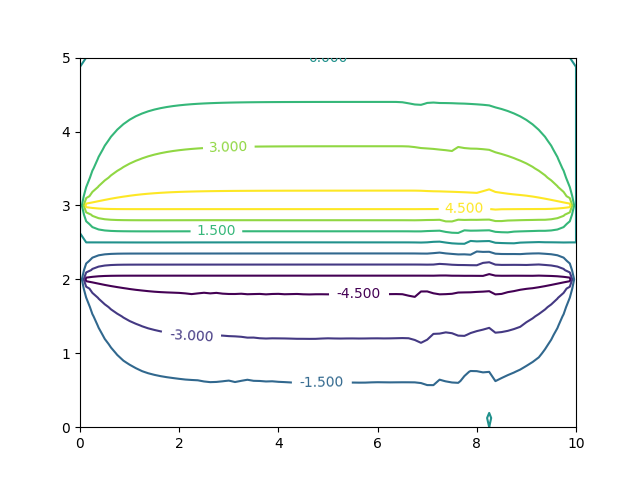
\includegraphics[scale=0.8]{imgs/cont_aprox_cap_1250.png}
    \caption{Mapa de linhas equipotenciais do sistema de capacitores}
    \label{cont_aprox_cap_1250}
\end{figure}

\begin{figure}[h!]
    \centering
    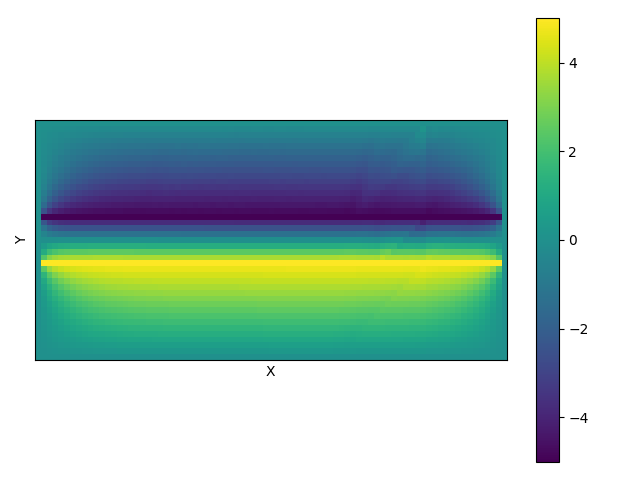
\includegraphics[scale=0.8]{imgs/hmap_aprox_cap_1250.png}
    \caption{Mapa de potencial do sistema de capacitores}
    \label{cont_aprox_cap_1250}
\end{figure}

\begin{figure}[h!]
    \centering
    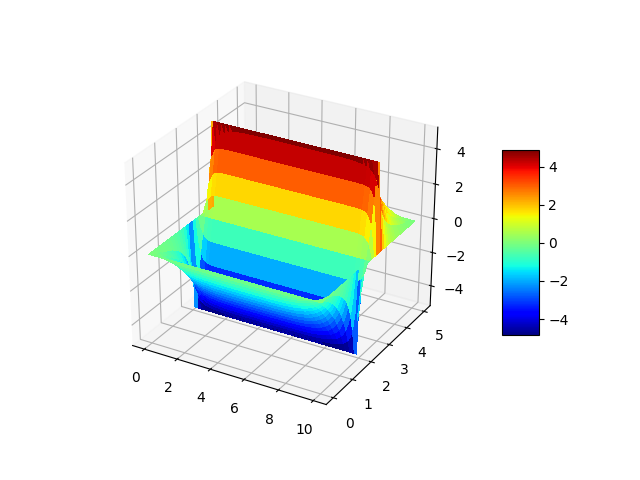
\includegraphics[scale=0.8]{imgs/3d_aprox_cap_1250.png}
    \caption{Mapa 3D do sistema de capacitores}
    \label{cont_aprox_cap_1250}
\end{figure}

Além disso, analisando o campo elétrico do capacitor:

\begin{figure}[h!]
    \centering
    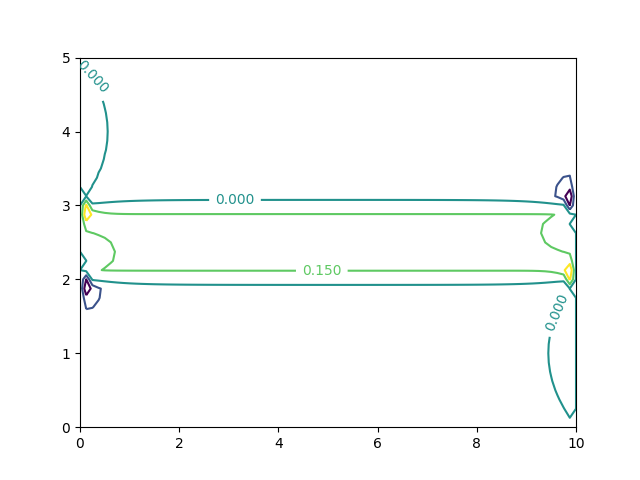
\includegraphics[scale=0.8]{imgs/cont_aprox_cap_elet_1250.png}
    \caption{Mapa 3d do campo elétrico do sistema de capacitores}
    \label{fig:my_label}
\end{figure}

\begin{figure}[h!]
    \centering
    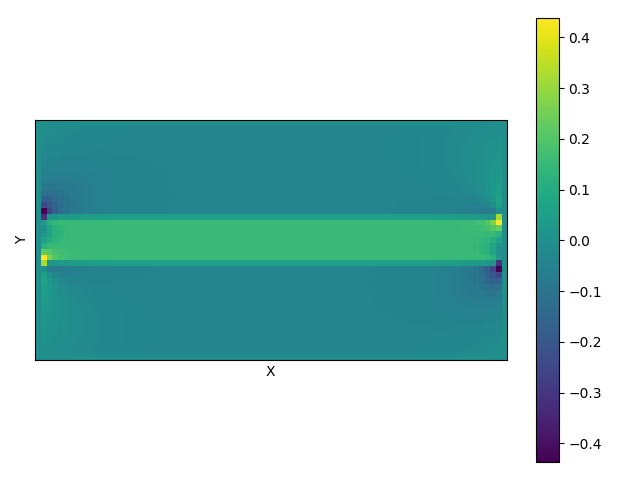
\includegraphics[scale=0.8]{imgs/hmap_aprox_cap_elet_1250.png}
    \caption{Mapa 3d do campo elétrico do sistema de capacitores}
    \label{fig:my_label}
\end{figure}

\begin{figure}[h!]
    \centering
    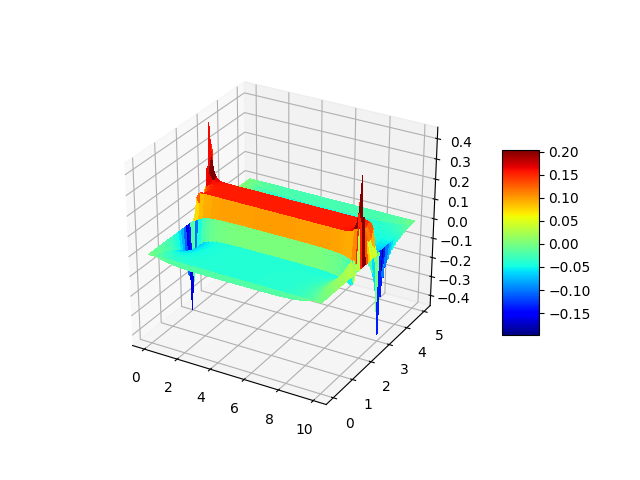
\includegraphics[scale=0.8]{imgs/3d_aprox_cap_elet_1250.png}
    \caption{Mapa 3d do campo elétrico do sistema de capacitores}
    \label{fig:my_label}
\end{figure}

\newpage
\newpage


\section{Documentação da classe} \label{sec_doc}
Abaixo consta a documentação do código desenvolvido ao longo do projeto. Conteúdo sobre algoritmos específicos se encontram dentro do próprio código, então o conteúdo abaixo é uma visão geral das propriedades da classe.
\subsection{Defines}
\begin{itemize}
    \item \texttt{MAX\_SIZE} \newline
        Tamanho máximo dos vetores $v, f, ground$. Deve ser \textbf{maior que} o valor de $n_x \cdot n_y$.
    \item \texttt{STD\_MAX\_ITER} \newline
        Máximo de iterações padrão do método SOR. Esse é o valor a ser utilizado caso não seja especificado um valor manualmente.
\end{itemize}
\subsection{Estruturas auxiliares}
\begin{itemize}
    \item \texttt{enum type} \newline
        Enum de tipos de problemas. Casos novos devem ser implementados aqui.
    \item \texttt{struct Dominio} \newline
        Struct auxiliar que descreve o domínio do problema atual.
\end{itemize}
\subsection{Atributos}
\begin{itemize}
    \item \texttt{dominio* dom} \newline
        Domínio do problema, definido pelo usuário.
    \item \texttt{int a, b, c, d, e} \newline
        Constantes do SOR, calculadas no construtor da classe.
    \item \texttt{int nx, ny} \newline
        Quantidade de passos em x e em y respectivamente, calculados no construtor da classe.
    \item \texttt{int hx, hy} \newline
        Tamanho dos passos em x e em y respectivamente, fornecidos pelo usuário.
    \item \texttt{double w}
        $\omega$ ideal, calculado conforme descrito na especificação.
    \item \texttt{double fp} \newline
        Vetor $f$, composto pela aplicação da função aproximante em todos os elementos do domínio.
    \item \texttt{double vp} \newline
        Vetor $v$, composto pela solução encontrada para o sistema.
    \item \texttt{double ground} \newline
        Vetor $ground$, composto pela solução exata do sistema. Calculado apenas quando uma função exata é fornecida.
    \item \texttt{double ground\_ep} \newline
        Vetor $ground$, composto pela solução exata do sistema em relação ao campo elétrico. Calculado apenas quando uma função exata é fornecida.
    \item \texttt{double (*aproxFunc) (double, double)} \newline
        Função aproximante. Deve receber 2 parâmetros do tipo double e retornar um parâmetro do tipo double.
    \item \texttt{double (*grndFunc) (double double)} \newline
        Função exata. Opcional. Deve receber 2 parâmetros do tipo double e retornar um parâmetro do tipo double.
    \item \texttt{std::vector<double (*) (double, double)> contornos} \newline
        Vetor de funções de contorno. Opcional. As funções devem receber 2 parâmetros do tipo double e retornar um parâmetro do tipo double. As funções devem ser aplicadas manualmente nas seções de contorno da implementação.
    \item \texttt{type t} \newline
        Tipo do sistema. Deve ser definido no enum \texttt{type}.
    \item \texttt{int vecSize} \newline
        Tamanho do vetor, dado por $nx * ny$.
    \item \texttt{double $erro\_{vp}$} \newline
        Erro cometido ao fim do processamento. Calculado no método \texttt{calcErr()}.
    \item \texttt{double erro\_ele} \newline
        Erro cometido ao fim do processamento em relação ao campo elétrico. Calculado no método \texttt{calcErrEsle()}.
    \item \texttt{int maxIter} \newline
        Número máximo de iterações permitidas no método SOR.
\end{itemize}
\subsection{Métodos}
reeeeeeeeee
\subsection{Extendendo a funcionalidade da classe}
Para extender a funcionalidade da classe, isto é, implementar novos tipos de problemas a serem resolvidos, primeiramente o cliente deve criar uma nova instância da classe \texttt{poissonSOR}, com o domínio e o passo desejados. Após isso, é necessário fornecer uma função de avaliação ao problema, isto é, a função $f(x, y)$ a ser calculada no domínio. Também é possível especificar um número máximo de iterações, por meio do método \texttt{setMaxIter()}. Caso não haja nenhum caso de contorno, isso já é o suficiente para utilizar a classe, chamando o método \texttt{process()} e analisando os resultados.
Caso seja necessário utilizar casos de contorno, é necessário, primeiramente, definir um novo tipo de problema no \texttt{enum type}, no cabeçalho da classe. Após isso, o cliente deve adicionar as funções de contorno por meio do método \texttt{addContorno()}. Com isso, o vetor de funções de contorno é preenchido apropriadamente. Após isso, o cliente deve alterar, na implementação da classe, as funções \texttt{checkContornos()}, \texttt{typeToString()} e \texttt{doSOR()}, adicionando uma cláusula ao sistema de \texttt{switch} já implementado. Com isso, os casos de contorno serão considerados nos cálculos. 
Assim, é possível implementar novos casos de teste rapidamente e de forma modularizada.
\chapter{Apêndice}
\section{Imagens}

\end{document}
